\documentclass[a4paper,12pt]{article}
\usepackage[left=1.5cm,right=1.5cm,
    top=1cm,bottom=1cm,bindingoffset=0cm]{geometry}

\usepackage[T1,T2A]{fontenc}
\usepackage[utf8]{inputenc}
\usepackage[english,russian,ukrainian]{babel}
\usepackage{tabularx}
\usepackage{amssymb}
\usepackage{color}
\usepackage{amsmath}
\usepackage{mathrsfs}
\usepackage{listings}
\usepackage{graphicx}
\graphicspath{ {./images/} }
\definecolor{lgreen}{rgb}{0.5,1,1}
\definecolor{n}{rgb}{1,0.5,0.5}



\begin{document}
\pagestyle{empty}
\begin{center}
   \begin{center} 
   \large{\textbf{Міністерство освіти і науки України} \par 
   \textbf{Національний технічний університет України}}\par
	“Київський політехнічний інститут”\par
	 Факультет електроніки\par
    	Кафедра мікроелектроніки\par
    \end{center}
    \vspace{4cm}
    
   	{\bfseries ЛАБОРАТОРНА РОБОТА № 1\par}
        \vspace{1cm}
        \large
        {
    	з курсу\par
    	«Теорія сигналів» \par
      	"Основи програмування мовою Python" \par  
	}
	\end{center}

       \vspace{7cm}
       \begin{tabularx}{\textwidth}{Xr}
        \flushright
           \begin{large} 
        Студента 3 курсу\par
 	групи ДП-82\par
	Мнацаканова Антона\par
	 \end{large}
	\end{tabularx}
   
   \vfill
   \begin{center}
    {Київ} --- 2020
    \end{center}
%-----------------------------------------------------------------------------------------------------    
    \newpage


\textbf{Завдання, частина 1.}\par
\fcolorbox{green}{lgreen}{4}. Ознайомитися з написанням власних файлів-сценаріїв. У власному файлі-сценарії побудувати графік лінійної функції однієї змінної. Позначити вісі та заголовок графіку, нанести координатну сітку.\par
\lstset{language=Python}          % Задаем язык исходного кода
\begin{lstlisting}    
#!/usr/bin/env python
#coding=utf8
from numpy import array, arange, abs as np_abs
import numpy as np
from math import sin, pi
import matplotlib.pyplot as plt
import matplotlib as mpl
import random
fig, ax = plt.subplots()
mpl.rcParams['font.family'] = 'fantasy'
mpl.rcParams['font.fantasy'] = 'Comic Sans MS, Arial'
x = np.linspace(1, 10, 50)
k = 3
b = 2
y = k*x + b
plt.title('Linear dependence y = kx+b') 
plt.xlabel('x')
plt.ylabel('y')
plt.grid(True)
plt.plot(x, y, "r")  
plt.show()
\end{lstlisting}
\vspace{1cm}\par
\fcolorbox{green}{lgreen}{5.1} Побудувати графіки синусоїд частот 1, 10, 50 Гц. Тривалість сигналів – 1 сек., частота дискретизації 256 Гц. Графіки будувати в одному вікні, але в різних осях. Амплітуди кожної синусоїди повинні бути випадковими числами.\par
\fcolorbox{green}{lgreen}{5.2} Виконати теж саме, але  задавати амплітуду кожної синусоїди з клавіатури.\par
\fcolorbox{green}{lgreen}{5.3} Підписати заголовок кожного графіку текстом, який буде містити значення частоти та амплітуди відповідної синусоїди.\par
\lstset{language=Python}          % Задаем язык исходного кода
\begin{lstlisting}    
from numpy import array, arange, abs as np_abs
from math import sin, pi
import matplotlib.pyplot as plt
import matplotlib as mpl
import random
mpl.rcParams['font.family'] = 'fantasy'
mpl.rcParams['font.fantasy'] = 'Comic Sans MS, Arial'

FD = 256
N = 256
F=1.0
w=(2.*pi*F/FD)
A=random.uniform(1,10)
\end{lstlisting}
\fcolorbox{red}{n}{(заміняємо всі ф-ї radom() на input()  для вводу значень з клавіатури)}
\lstset{language=Python}
\begin{lstlisting}  
plt.subplot(3,1,1) 
sin_sig = array([A*sin(w*t) for t in range(N)])
plt.plot(arange(N)/float(FD), sin_sig, 'r')
plt.xlabel('Time, s')
plt.ylabel('Applitude = '+  str("{0:.2f}".format(A) ))
plt.title('Sin signal, Frequency = ' +  str("{0:.2f}".format(F) ))
plt.grid(True)
plt.hold(True)
FD = 256
N = 256 
F=10.0
w=(2.*pi*F/FD)
A=random.uniform(1,10) 
plt.subplot(3,1,2) 
sin_sig = array([A*sin(w*t) for t in range(N)])
plt.plot(arange(N)/float(FD), sin_sig, 'r')
plt.xlabel('Time, s')
plt.ylabel('Applitude = '+  str("{0:.2f}".format(A) ))
plt.title('Sin signal, Frequency =' +  str("{0:.2f}".format(F) ))
plt.grid(True)
plt.hold(True)
FD = 256
N = 256
F=50.0
w=(2.*pi*F/FD)
A=random.uniform(1,10)
plt.subplot(3,1,3) 
sin_sig = array([A*sin(w*t) for t in range(N)])
plt.plot(arange(N)/float(FD), sin_sig, 'r')
plt.xlabel('Time, s')
plt.ylabel('Applitude = '+  str("{0:.2f}".format(A) ))
plt.title('Sin signal, Applitude = ' +  str("{0:.2f}".format(F) ))
plt.grid(True)
plt.hold(True)
plt.show()
\end{lstlisting}
\begin{center}
\includegraphics[height = 11.5 cm,width=13 cm]{a.png}
\end{center}
%-----------------------------------------------------------------------------------------------------    
    \newpage
\fcolorbox{green}{lgreen}{6.}  Ознайомитися з роботою функцій, що генерують прямокутні імпульси, гаусівські імпульси, трикутні імпульси та послідовності імпульсів заданої форми.\par
\fcolorbox{green}{lgreen}{6.1} Побудувати одиночний прямокутний імпульс. Задати проміжок значень часу 10 секунд, частота дискретизації 256 Гц. Побудувати графік одиничного прямокутного імпульсу шириною 300 мс, з центром в момент часу 4 с.\par
\lstset{language=Python}
\begin{lstlisting}  
from numpy import array, arange, abs as np_abs
from math import sin, pi
import matplotlib.pyplot as plt
import matplotlib as mpl
import random

mpl.rcParams['font.family'] = 'fantasy'
mpl.rcParams['font.fantasy'] = 'Comic Sans MS, Arial'

fd = 256.0
t_min = 0
t_max = 10
delta_t = 1.0/fd;
A = 5
b = 0.3
a = 4.0 - b/2;

def f(x):
    if x < a:
        return 0;
    if x < a+b:
        return A;
    return 0;

x = [];
y = [];
t = t_min;
while t<=t_max:
    x.append(t);
    y.append(f(t));
    t += delta_t

    
plt.plot(x, y, 'r')
plt.xlabel('Time, s')
plt.ylabel('Applitude')
plt.title('Square wave')
axes = plt.gca()
axes.set_xlim([-1,11])
axes.set_ylim([-1,6])
plt.grid(True)
plt.show()
\end{lstlisting}
\begin{center}
\includegraphics[height = 11.5 cm,width=15 cm]{6.1.png}
\end{center}
\fcolorbox{green}{lgreen}{6.2} Написати файл-сценарій для побудови графіку прямокутного імпульсу, тривалість та амплітуда якого буде задаватися з клавіатури. Розташування імпульсу задавати випадковим числом, але передбачити перевірку, чи не виходе імпульс за межі графіка.
\lstset{language=Python}
\begin{lstlisting}
#!/usr/bin/env python
#coding=utf8

from numpy import array, arange, abs as np_abs
from math import sin, pi
import matplotlib.pyplot as plt
import matplotlib as mpl
import random
mpl.rcParams['font.family'] = 'fantasy'
mpl.rcParams['font.fantasy'] = 'Comic Sans MS, Arial'

fd = 256.0
t_min = -0.5
t_max = 10.5
delta_t = 1.0/fd;

print ('Amplitude:')
A = input()
print ('Pulse Width((0;10]): ')
b = input()
a = random.uniform(0,10-b)

if b>10:
	print ("Impulse outside the schedule!")
	exit()
def f(x):
    if x < a:
        return 0;
    if x < a+b:
        return A;
    return 0;

x = [];
y = [];
t = t_min;
while t<=t_max:
    x.append(t);
    y.append(f(t));
    t += delta_t
 
plt.plot(x, y, 'r')
plt.xlabel('Time, s')
plt.ylabel('Amplitude')
plt.title('Square wave')
plt.grid(True)
axes = plt.gca()
axes.set_xlim([-1,11])
axes.set_ylim([-1,A+1])
plt.show()
\end{lstlisting}
\begin{center}
\includegraphics[height = 12 cm,width=15 cm]{6.2.png}
\end{center}

\fcolorbox{green}{lgreen}{6.3} Побудувати послідовність прямокутних імпульсів для двох випадків: а) коли інтервали між імпульсами однакові, б) коли інтервали між імпульсами випадкові і задаються програмно.
\lstset{language=Python}
\begin{lstlisting}
from numpy import array, arange, abs as np_abs
from math import sin, pi
import matplotlib.pyplot as plt
import matplotlib as mpl
import random
mpl.rcParams['font.family'] = 'fantasy'
mpl.rcParams['font.fantasy'] = 'Comic Sans MS, Arial'

fd = 256.0
t_min = -0.5
t_max = 100.5
delta_t = 1.0/fd;
print ('Maintain the amplitude: ')
A = input()
print ('Enter the impulse width( (0;10] ): ')
b = input()
print ('Enter the intervals between impulses: ')
a = input()
#a = random.uniform(0,10-b)
if b>10:
	print ("Impulse outside the schedule")
	exit()
def f(x,imp_begin,imp_width):
    if x < imp_begin:
        return 0;
    if x < imp_begin+imp_width:
        return A;
    return 0;
    
x = [];
y = [];
t = t_min;
while t<=t_max:
    aa = t
    bb = t + a + b
    cc = t+a
    while aa<=bb:
        x.append(t);
        y.append(f(t,cc,b));
        aa += delta_t
        t += delta_t

x1 = [];
y1 = [];
t = t_min;
while t<=t_max:
    aa = t
    aaa = random.uniform(1,5)
    bb = t + aaa + b
    cc = t+aaa
    while aa<=bb:
        x1.append(t);
        y1.append(f(t,cc,b));
        aa += delta_t
        t += delta_t

plt.subplot(2,1,1)  
plt.plot(x, y, 'r')
plt.xlabel('Time, s')
plt.ylabel('Amplitude')
plt.title('Square wave(intervals between pulses are the same)')
plt.grid(True)
axes = plt.gca()
axes.set_xlim([-1,101])
axes.set_ylim([-1,A+1])
plt.hold(True)

plt.subplot(2,1,2)  
plt.plot(x1, y1, 'g')
plt.xlabel('Time, s')
plt.ylabel('Amplitude')
plt.title('Square wave(intervals between pulses are random)')
plt.grid(True)
axes = plt.gca()
axes.set_xlim([-1,101])
axes.set_ylim([-1,A+1])
plt.hold(True)
plt.show()
\end{lstlisting}
\begin{center}
\includegraphics[height = 12 cm,width=15 cm]{6.3.png}
\end{center}




\fcolorbox{green}{lgreen}{7} Зберегти дані розрахунку функції в файл. Прочитати їх із файлу в іншому сценарії, побудувати графік функції.
\lstset{language=Python}
\begin{lstlisting}
#!/usr/bin/env python
#coding=utf8
import numpy as np
import matplotlib.pyplot as plt
ex_2 = np.load('example_2.npz')
ex_2.files
x = ex_2['arr_0']
y = ex_2['arr_1']
A = ex_2['arr_2']

plt.plot(x, y, A, 'r')
plt.xlabel('Time, s')
plt.ylabel('Amplitude')
plt.title('Square wave(readen from file)')
plt.grid(True)
axes = plt.gca()
axes.set_xlim([-1,11])
axes.set_ylim([-1,A+1])
plt.show()
\end{lstlisting}
%\begin{center}
%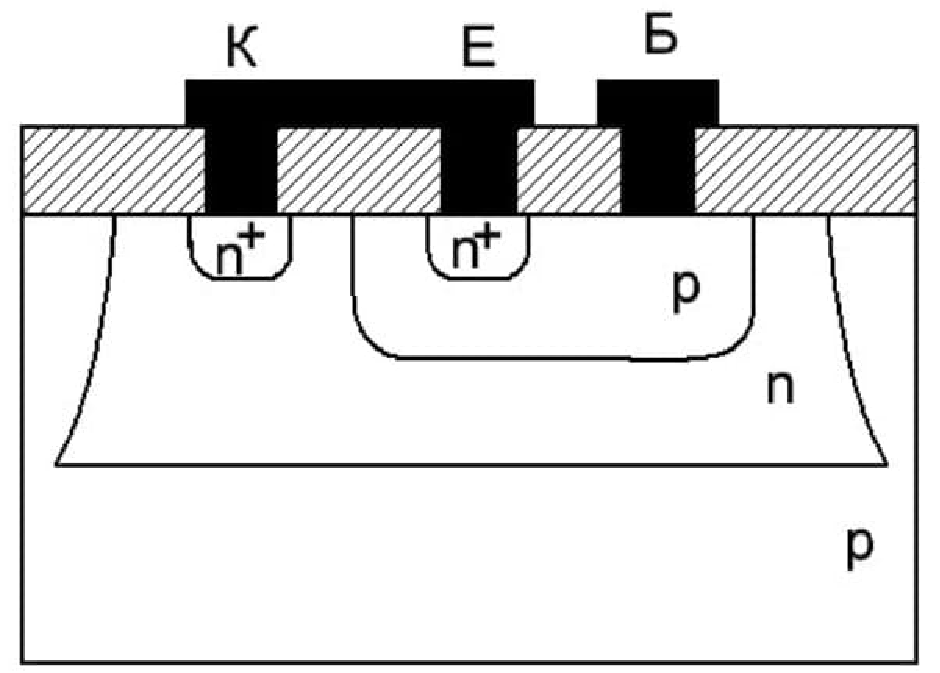
\includegraphics[height = 12 cm,width=15 cm]{7.png}
\hoffset=-6mm{
\begin{figure}[h]
\begin{minipage}[h]{0.49\linewidth}
{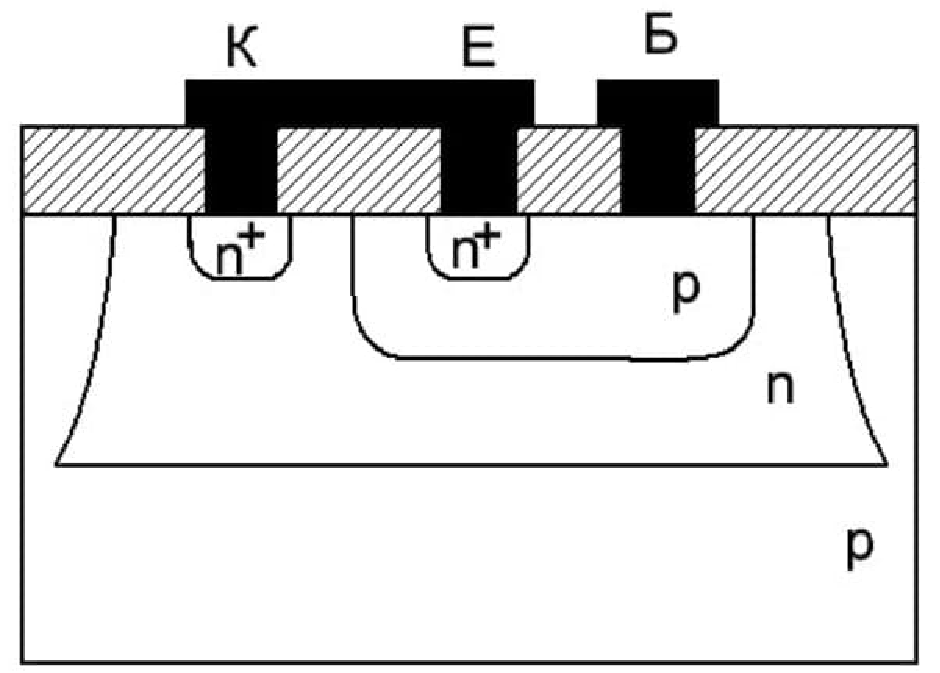
\includegraphics[height = 7 cm,width=10 cm]{7.png} }
\end{minipage}
\hfill
\begin{minipage}[h]{0.49\linewidth}
{\includegraphics[height = 7 cm,width=10 cm]{7_readen.png} }
\end{minipage}
\end{figure}
}
%\end{center}




\end{document}